%!TEX root = Presentation-Thoma.tex

\section{Szenario}
\subsection{Semantische Segmentierung}
\begin{frame}{Pixelweise Semantische Segmentierung}
    \begin{figure}[ht]
        \begin{minipage}[b]{0.45\linewidth}
            \centering
            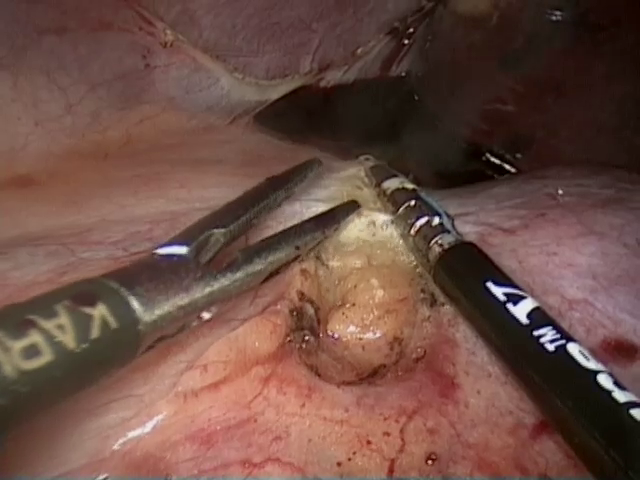
\includegraphics[width=\textwidth]{../images/img_35_raw.png}
            \caption{[Maier-Hein et al, 2014]\hspace{\textwidth}Input}
            \label{fig:input}
        \end{minipage}
        \hspace{0.5cm}
        \begin{minipage}[b]{0.45\linewidth}
            \centering
            
\includegraphics[width=\textwidth]{../images/img_35_label.png}
            \caption{[Maier-Hein et al, 2014]\hspace{\textwidth}Label / Output}
            \label{fig:label}
        \end{minipage}
    \end{figure}
\end{frame}

\begin{frame}{Semantische Segmentierung}
    \begin{figure}[ht]
        \begin{minipage}[b]{0.45\linewidth}
            \centering
            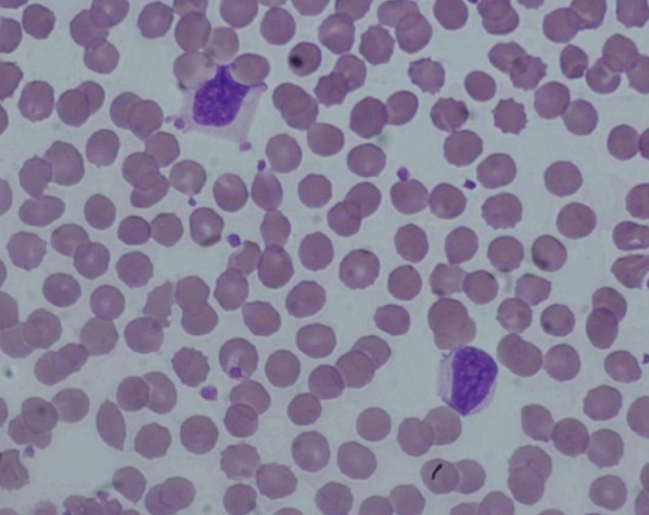
\includegraphics[width=\textwidth]{../images/red-blood.png}
            \caption{[Sharif 2012] Rote Blutkörperchen}
            \label{fig:red-blood}
        \end{minipage}
        \hspace{0.5cm}
        \begin{minipage}[b]{0.45\linewidth}
            \centering
            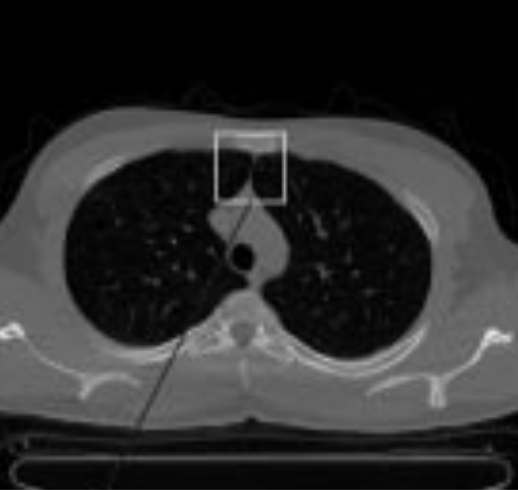
\includegraphics[width=\textwidth]{../images/lung.png}
            \caption{[Hu 2001] Lunge}
            \label{fig:lung}
        \end{minipage}
    \end{figure}
\end{frame}

\begin{frame}{Semantische Segmentierung}
    \begin{figure}[ht]
        \begin{minipage}[b]{0.45\linewidth}
            \centering
            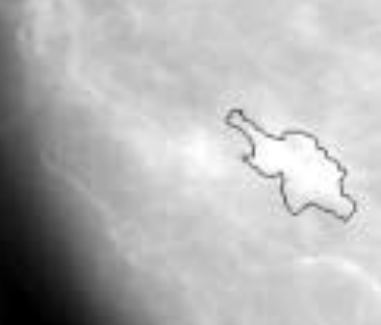
\includegraphics[width=\textwidth]{../images/mammography.png}
            \caption{[Pham 2000] Mammographie}
            \label{fig:mammographie}
        \end{minipage}
        \hspace{0.5cm}
        \begin{minipage}[b]{0.45\linewidth}
            \centering
            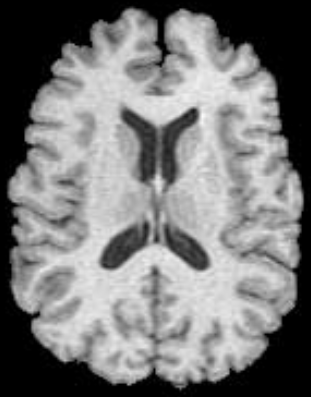
\includegraphics[width=\textwidth]{../images/brain-mr.png}
            \caption{[Pham 2000] Gehirn}
            \label{fig:lung}
        \end{minipage}
    \end{figure}
\end{frame}
